

\section{Compressed Baryonic Matter experiment, subdetectors and their tasks}
The Compressed Baryonic Matter (\gls{CBM}) experiment is currently being constructed at \gls{FAIR}. Figure~\ref{fig:exp} depicts the CAD drawing of the \gls{CBM} experiment. The beam enters the experimental cave from the left side and traverses the High Acceptance Di-Electron Spectrometer (\gls{HADES}) experiment to finally reach the target of the \gls{CBM} experiment. 

\begin{figure}[!h]
    \centering
    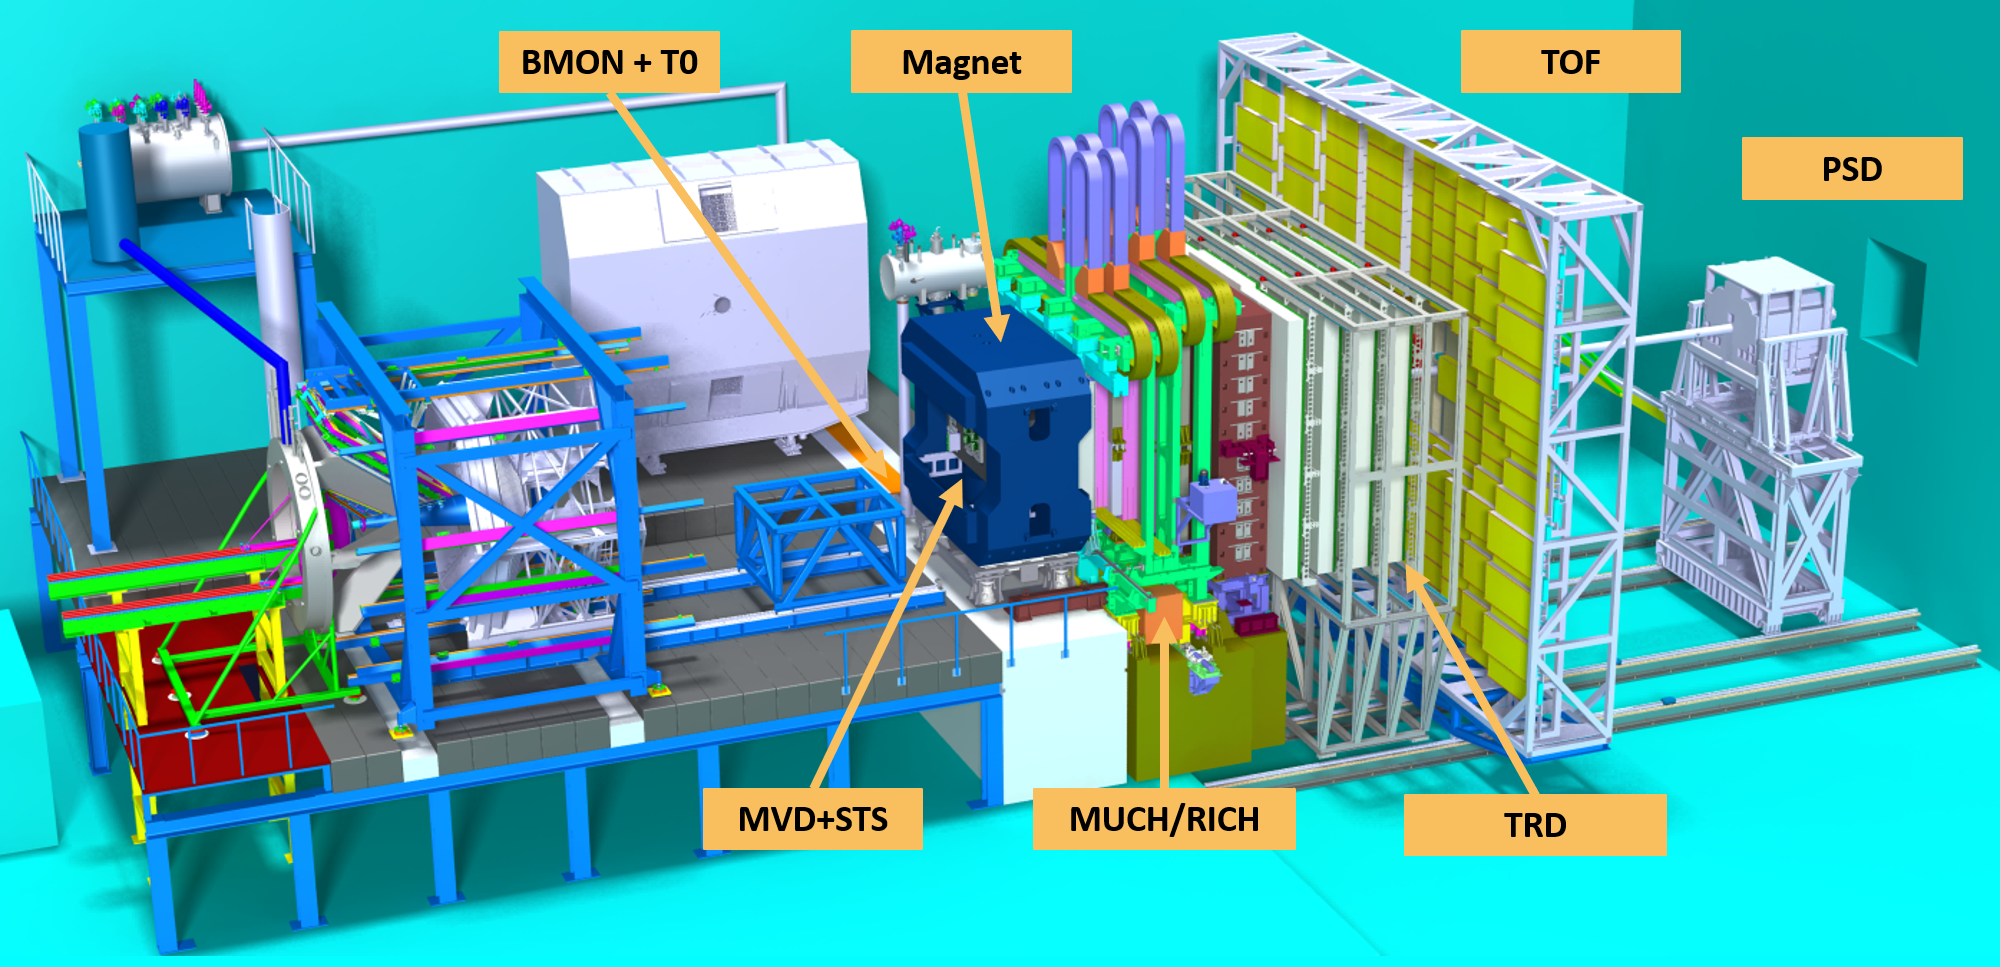
\includegraphics[width=1\columnwidth]{Chapter1/images/CBMnew.png}
    \caption{HADES experiment on the left side and the \gls{CBM} experiment on the right side.}
    \label{fig:exp}
\end{figure}

The main features of the experiment are described below:
\begin{itemize}
\item Tracking acceptance: $\SI{2.5}{\degree} < \theta_{lab} < \SI{25}{\degree}$
\item Peak event intensities up to $10\,\mathrm{MHz}$ for Au+Au systems
\item Fast and radiation hard detectors
\item Free-streaming triggerless Data Acquisition (\gls{DAQ})
\item 4D tracking (spatial and time)
\item Online event reconstruction and selection
\item Data rates from the readout electronics of up to 2~\,TB/s
\end{itemize}


In order to get valuable insight into the physics observables proper detector systems need to be developed. The detector concept is based on identifying the stable charged particles that are often decay products of resonances and unstable particles. Charged particles can be bent in a magnetic field of known strength to investigate their momentum. Together with information from Time-of-flight (\gls{TOF}) the mass of particles can be distinguished. Di-leptons are considered special due to their nature. They may contain undisturbed information from the early, dense phase of the fireball evolution. On the other hand, it is necessary to separate them from the abundant pions. In order to perform the complete analysis, the following detector systems are foreseen for the \gls{CBM} experiment:\bigbreak


\textbf{Beam monitor, or T0 (\gls{BMON})} and its conceptual design, was summarized during the 40th \gls{CBM} Collaboration Meeting~\cite{bmon}. Two separate stations in front of the target are made out of high-purity poly-crystalline CVD diamond material. This detector is foreseen to monitor beam quality (position, time structure) and determine the start time of the reaction.\bigbreak

\textbf{Micro Vertex Detector} (\gls{MVD}) consists of four planar stations with Monolithic Active Pixel Sensor (\gls{MAPS}) chips. A station layout and distance from the target can be tailored to the needs of a specific run, for example, to optimize vertexing or tracking. The vertexing detector geometry aims at a precision of secondary vertices determination of about $50$ -- \mum{100} along the beam axis. The main aim is decay vertex identification of the very short-lived particles such as charmed mesons, which decay within a few hundred \SI{}{\micro\metre} behind the target, as well as background rejection in di-electron spectroscopy~\cite{MVD}.\bigbreak

 \textbf{Silicon Tracking System} (\gls{STS}) which is responsible for tracking charged particles inside the magnetic field. The \gls{STS} is located inside a superconducting dipole magnet~\cite{Malakhov:109025}. The charged particles traversing the active volume of \gls{STS} are bent due to the applied magnetic field. The trajectories of charged particles inside the magnetic field will be determined by MVD and STS across a \SI{1}{\metre} length downstream of the target~\cite{Heuser:54798}.\bigbreak
 
\textbf{Muon Chamber System} (\gls{MUCH}) is the fourth subsystem of the \gls{CBM} experiment. It is dedicated to muon detection (for example rare particles decaying into muons like $J/\psi$) and track reconstruction. This concept is based on the layered design of the hadron absorbers ($5$ layers), separated with tracking detector planes which are based on Gas Electron Multiplication (\gls{GEM}) and Resistive Plate Chambers (\gls{RPC}) detectors~\cite{MUCH}.\bigbreak

\textbf{Ring Imaging Cherenkov Detector} (\gls{RICH}) is responsible for electron identification via Cherenkov radiation~\cite{RICH}. The detector consists of \SI{1.7}{\metre} a long $\mathrm{CO_{2}}$ gas radiator with pion threshold for Cherenkov radiation of \agevc{4.65}, two arrays of mirrors, and photon detector planes. It allows separating electrons from pions up to \agevc{8}. The models predict that a pion suppression on the level of $500$ will be accomplished thanks to the high granularity (about $55000$ channels) and high number of photons per ring~\cite{RICH}.\bigbreak

\textbf{Transition Radiation Detector} (\gls{TRD}) suppresses pions and  supports track reconstruction with 9-10 detector layers grouped into $3$ stations. It is placed between \SI{4}{\metre} to \SI{9}{\metre} downstream of the target, and the total active area reaches \SI{600}{\square\metre}. Because the RICH electron identification capabilities are limited to the lower momentum range ($p < $~\agevc{5}), the TRD will be employed as a supplementary device to supplement and expand the electron identification into higher momenta. The TRD configuration designed for the SIS100 CBM setup will therefore be capable of identifying electrons beyond a momentum threshold of $p > $~\agevc{1} with a $90$\% efficiency while reducing the hadronic background by a factor of $10 - 20$. The working principle of the detector is based on the phenomenon that the ultra-relativistic particles traversing through a medium with alternating dielectric constant produce transition radiation. It is composed of two parts, the readout chamber, and the radiator. The photons are generated by the electrons passing through the radiator, while the heavier pions do not produce any radiation. For detection of the produced radiation, multi-wire proportional chambers will be used with a $85\%\,\mathrm{Xe}/\,15\%\,\mathrm{CO_{2}}$ gas mixture)~\cite{TRD}. \bigbreak

\textbf{Time-of-Flight Detector} (\gls{TOF}) is designed to identify hadrons (pions, kaons, and protons). As the name indicates, the detector measures the time-of-flight of the reaction products with Multi-Gap Resistive-Plate Chambers (\gls{MRPC}). The \glspl{MRPC} have an excellent time resolution of \SI{60}{\pico\second}.  It might be located between \SI{6}{\metre} and \SI{10}{\metre} (depending on the physics objectives) and will cover an area of about \SI{120}{\square\metre}~\cite{TOF}. \bigbreak

\textbf{Projectile Spectator Detector} (\gls{PSD}) is the last subsystem of the \gls{CBM} experiment, and it determines the collision centrality and event plane. The detector is meant to measure the nucleons from a projectile nucleus in heavy-ion collisions. The proposed $44$ module design of the PSD covers a large transverse area around the beam spot position, such that most of the projectile spectator fragments deposit their energy in the \gls{PSD}. The detector concept is a compensating hadron calorimeter consisting of lead-scintillator sandwich modules~\cite{PSD}.\bigbreak


The CBM detector system can be used in two operation modes: the first one is optimized for electron identification (electron configuration) and the second is designed for muon identification (muon configuration). In the first one, all the subsystems apart from MUCH will be involved. In the muon configuration, the \gls{RICH} detector is replaced by \gls{MUCH}.

For the high-rate CBM experiment, the triggerless data read-out and acquisition system plays a crucial role. The time-stamped signals will be read out without event correlation and transferred to a high-performance computing farm, the GSI GreenIT Cube. The online event reconstruction and selection will be performed by high-speed algorithms. In the first step, the tracks of the charged particles are reconstructed from the space and time information from the various detector signals. This process is based on the Cellular Automaton (\gls{CA}) track finder~\cite{CA}. Subsequently, the particles are identified, taking into account secondary decay vertices and information from \gls{RICH} or \gls{MUCH}, \gls{TRD}, and \gls{TOF}. Finally, the particles are grouped into events, which will be selected for storage if they contain important observables. In parallel, the event and its plane are characterized using information from the PSD.

Another important online system is called Experiment Control System (\gls{ECS}). It is a software structure that aims to provide automatization, monitoring, and control of hardware and the detector subsystems. A detailed description of \gls{ECS} and the detector-specific control system (\gls{DCS}) will be given in Chapter~\ref{chap:online_systems}.



\section{Thesis overview and its rationale}
The thesis consists of seven chapters. The second chapter introduces the role of silicon trackers in large scientific experiments and discusses the design details of \gls{STS}, including the physics performance and experimental challenges. Those elements define the requirements for the Detector Control System (\gls{DCS}). The third chapter serves as an introduction to the control and monitoring of a large experiment, with an extended focus on the detector-related slow control system and the developed control framework. The following three chapters are focused on the results and their consequences for the experiment:
\begin{itemize}
    \item Chapter $4$ covers the first implementations of the mentioned control framework. The first application is related to the slow control interface for the Front-End Electronics (\gls{FEE}) readout. The second and third examples are related to the irradiation studies of the powering modules for the Low Voltage (\gls{LV}) powering of \gls{STS} electronics and thermal cycling of Front-end boards (\glspl{FEB}). The performed studies and results of these activities are discussed in detail.
    \item Chapter $5$ describes the efforts to design and test a distributed sensing system for \gls{STS} with a focus on humidity sensing. Three considered technologies feature capacitive sensors, fiber optic sensors, and remote sensing with the use of a sampling system. The chapter focuses on the design choices and characterization of the fiber Bragg grating-based sensors. 
    \item Chapter $6$ focuses on controlling a small-scale prototype version of \gls{STS} in the \gls{mCBM} experiment. The first sections describe in detail the hardware and software solutions implemented in the detector. Subsequently, the results from the full-blown \gls{DCS} are presented and discussed, including the radiation effects on the silicon sensors and general considerations about the power dissipation of different elements of \gls{STS} powering scheme. Moreover, considerations about the \gls{DCS} are given. 
\end{itemize}
The last part of the thesis summarizes the results and sheds light on the next steps toward the realization of \gls{STS} and its controls. The most important findings and results from the performed studies are also discussed.